This section is dedicated to describing the general concept of the new readout-system. 
The system was given the name \gls{theresa} and in the sections to follow, this name will be used to denote the new system.

First, a short overview of state of the art systems is given, including commercially available real-time oscilloscopes and \gls{kapture}.
This system was developed at the \gls{ipe} at \gls{kit} specifically addressing the needs of \gls{thz} diagnostics at \gls{kara}.
The working principle of this system is explained in detail, as the new \gls{theresa} system is an evolution of the \gls{kapture} system. 

Then, the architecture of the \gls{theresa} system itself is described.

\section{State Of The Art Readout-Systems}
In this section first a short overview over commercially available real-time oscilloscopes and their performance is given. 
Then, the \gls{kapture} system, which is in operation at \gls{kara}, is presented in detail.
\subsection*{Real-Time Oscilloscopes}
Real-time oscilloscopes are defined by three key specifications: bandwidth, sample rate, and memory depth.
Some examples of currently commercially available oscilloscopes are listed in \autoref{tab:real_time_osc}.
The acquisition time is given for the case of maximal sample rate.
It can be calculated as 
\begin{equation}
	\text{Acquisition Time} = \frac{\text{Memory Depth}}{\text{Max. Sample Rate}}
\end{equation}
As can be derived from the table, the acquisition time of such oscilloscopes is quite limited, not allowing for continuous sampling of fast input signals.
\begingroup
\renewcommand{\arraystretch}{1.5}
\begin{table}[tb]
	\caption[Real Time Oscilloscopes Examples]{Some example real-time oscilloscopes with (max.) key characteristics}
	\label{tab:real_time_osc}
	\centering
	\begin{tabularx}{\textwidth}{Xcccc}
		%todo to num und s-column %todo größerem zeiekabstand\toprule
		\textbf{Model}            & \textbf{Bandwidth} &         \textbf{Sample Rate}         &  \textbf{Memory Depth}  & \textbf{Acquisition time} \\ \midrule
		Keysight MXR608A          &    \SI{6}{\GHz}    & \SI{16}{\giga \sample \per \second}  & \SI{1.6}{\giga \sample} &  \SI{10}{\milli \second}  \\
		Tektronix DPO70000SX      &   \SI{70}{\GHz}    & \SI{200}{\giga \sample \per \second} &  \SI{1}{\giga \sample}  &  \SI{5}{\milli \second}   \\
		LeCroy LabMaster 10-100Zi &   \SI{65}{\GHz}    & \SI{160}{\giga \sample \per \second} & \SI{512}{\mega \sample} & \SI{3.2}{\milli \second}  \\ \bottomrule
	\end{tabularx}
\end{table}
\endgroup

\subsection{KAPTURE}
\Gls{kapture} (Karlsruhe Pulse Taking Ultra-Fast Readout Electronics) is a fast readout system developed at the \gls{ipe} for \gls{thz} diagnostics at \gls{kara}. 
It is designed to digitize the pulses generated by \gls{thz} detectors at each electron bunch revolution, with a memory-efficient approach to acquire the detector signal on a bunch-by-bunch basis (sampling only the pulses themselves). 
The system is able to sample pulses with a \gls{fwhm} between a few tens to a hundred picoseconds with a minimal sample time of \SI{3}{\pico \second}. \cite{caselleKAP}

To showcase the revolution of this \gls{daq} system, the general architecture and concept is explained with the first version of \gls{kapture}.
Then, the improved version \gls{kapture2} is presented.
At the end, being a further evolution of these two versions, the architecture of \gls{theresa} is explained.

\subsubsection*{General Concept}
The system consists of two parts: the sampling front-end card and a \gls{fpga} readout card. In \autoref{fig:thz_chain} the setup for \gls{thz} radiation measurements with \gls{kapture} is shown. 

The incoming radiation is fed into a detector, which converts the incident photons into an electrical signal. 
This signal is then amplified in a wide-band \gls{lna}. 
A wideband lossless power splitter, developed at \gls{ipe}, splits the detector signal into four identical signals, which are then propagated to the sampling front-end card. 
The card consists of four parallel sampling channels with adjustable sampling time. 
Each channel contains a \gls{tha} and an \gls{adc}. 
This card is connected to a read-out card by a high-speed and high-density connector. 
The \gls{fpga} sets the sampling time for each individual sampling channel and reads, processes and sends all acquired data to a \gls{cpu}/\gls{gpu} cluster for further processing. \cite{caselle2014}

\begin{figure}[tb]
	\centering
	\includegraphics[width = \textwidth]{chap/03-newSys/img/kapture/thzChain.tikz}
	\caption[THz measurement with KAPTURE]{\gls{thz} radiation measurement setup with \gls{kapture} (redrawn from \cite{caselle2014})}
	\label{fig:thz_chain}
\end{figure}

\paragraph{Analog Front-End}
Due to the high bandwidth nature of the detector signal, the analog front-end of the system has to be wideband as well to be able to sample the signal with picosecond resolution. 

The used \gls{lna} is based on a commercial GaAs \gls{mmic} which operates from \gls{dc} to \SI{50}{\giga \hertz}. 
It is needed to compensate the insertion loss\footnote{\textit{Insertion loss} is the loss of signal power which occurs, when a signal passes through a component.} of the following power-splitter stage. 
Classical power-splitters are not intrinsically wideband (see \cite{caselle2014}). 
For that reason, an wideband power-splitter was developed at \gls{ipe} which fulfills the bandwidth requirements. 
The designed power-splitter works up to \SI{100}{\giga \hertz} with an insertion loss of \SI{8}{\decibel} (at \SI{100}{\GHz}) and a return loss\footnote{\textit{Return loss} is the loss of signal power due to reflection by a discontinuity in the transmission line.} of about \SI{20}{\decibel} at \SI{50}{\giga \hertz}. \cite{caselle2014}
A photo of the power-splitter is shown in \autoref{fig:power_splitter}.

\begin{figure}[tb]
	\centering
	\includegraphics[width = 0.6\textwidth]{chap/03-newSys/img/kapture/power_split}
	\caption{Photo of the power-splitter developed at IPE}
	\label{fig:power_splitter}
\end{figure}

\paragraph{Sampling Board}
The archtiecture of the front-end board with the power-splitter is shown in \autoref{fig:kapture}. 
\begin{figure}[tb]
	\centering
	\includegraphics[width = \textwidth]{chap/03-newSys/img/kapture/kapture.tikz}
	\caption[General architecture of the KAPTURE system]{General architecture of the \Gls{kapture} front-end sampling card (cf. \cite[p.2]{caselleKAP})}
	\label{fig:kapture}
\end{figure}

The power-splitter splits the incoming signal into four identical signals, which are then fed into four parallel channels, consisting of a respective \gls{tha} unit and a 12-bit \gls{adc} sampling at \SI{500}{\mega\sample\per\second}. 
The sampling time of each unit can be adjusted individually with a delay chip with a resolution of \SI{3}{\pico \second} (maximal delay range: \SI{100}{\pico \second}). 
The delay chips are programmed with the \gls{fpga} on the readout card.
The clock signal is provided by \gls{kara}, which is cleared from jitter by a \gls{pll}. 
This ensures the synchronization of the \glspl{adc} with the \gls{rf} system. 
The cleaned clock signal is distributed to the delay chips via fan-out buffer \cite{caselleKAP}.
In this way, the pulse can be ``locally sampled'' by adjusting the different delay with a maximum rate of \SI{330}{\giga\sample\per\second} possible. 
A simplified representation of the local sampling of the signal is shown in \autoref{fig:sig_kap1_kap2}.
The plot shows on the left the sampling of the signal for \gls{kapture} and on the right for \gls{kapture2} (described below).
The sampling points $S_n$ are acquired by setting the respective delay $\Delta t_n$ of the sampling times. 
\begin{figure}[tb]
	\centering
	\begin{subfigure}{0.48\textwidth}
		\centering
		\includegraphics[width=0.8\textwidth]{chap/03-newSys/img/kapture/signal_kap1.tikz}  
		\label{fig:sig_kap1}
	\end{subfigure}
	\hfill
	\begin{subfigure}{0.48\textwidth}
		\centering
		\includegraphics[height=0.8\textwidth]{chap/03-newSys/img/kapture/signal_kap2.tikz}  
		\label{fig:sig_kap2}
	\end{subfigure}
	\caption[KAPTURE Pulse Sampling]{Sample points $S_n$ acquired by setting the sampling delay times $\Delta t_n$ accordingly. Left plot shows pulse sampled by KAPTURE v1, right by KAPTURE v2}
	\label{fig:sig_kap1_kap2}
\end{figure}

\paragraph{GPU-DAQ System}
The sampling system produces a large amount of data.
In order to keep a continuous data  acquisition the necessary bandwidth is 
\begin{equation}
	12\;\text{bits} \cdot 8 \; \text{samples} \cdot \SI{1}{\GHz} = \SI{96}{\giga \bits \per \second}
\end{equation}
To ensure high data throughput, a high-speed \gls{pcie} readout card was developed (called ``High-Flex'') was developed.
This card receives the samples and tags them with the respective bunch identification. 
The data is then sent to a \gls{gpu} using a \gls{pcie} connection based on direct \gls{fpga}-\gls{gpu} direct memory access architecture.
The \gls{gpu} node reconstructs the pulse based on the given sampling points and calculates the amplitude and pulse arrival time. 
It also performs an online \gls{fft} for frequency analysis.
To store the data temporary before it is sent to the \gls{daq} system, a large \gls{ddr3} memory device is used, as seen in \autoref{fig:kapture}. \cite{caselleKAP}

\subsection{KAPTURE-2}
The first version of \gls{kapture} has a limitation concerning the number of sampling points per pulse and does not allow to sample the baseline of the detector.
Analyzing the baseline however is very important, as it is changing slightly and affects the pulse amplitude of the bunch. 
Due to this distortion, calculating the correlation between bunches was limited. 
For this reason, a second version of \gls{kapture} was designed in order to overcome these limitations. 
The \gls{pll} on the sampling board allows for synchronization between two or more \glspl{pll} located on different boards.
With this feature, the sampling time of two boards can be synchronized and in this way extend the number of sampling points beyond four.
A comparison of the sampling concepts is shown in \autoref{fig:kap1_vs_kap2}.

In \gls{kapture2}, two front-end boards can be connected to directly sample the pulses with up to eight sampling point at the pulse repetition rate \SI{2}{\GHz}. 
Alternatively, the system can sample the pulse and the baseline between two consecutive pulses with a constant pulse rate up to \SI{1}{\GHz} (see \autoref{fig:kap2}).
In this way, the read-out card can calculate the correct amplitude of the pulse and send it to the \gls{gpu} for further processing \cite{caselleKAP}.

\begin{figure}[tb]
	\centering
	\begin{subfigure}{0.48\textwidth}
		\centering
		\includegraphics[width=0.8\textwidth]{chap/03-newSys/img/kapture/kap1.tikz}  
		\caption{Sampling concept in KAPTURE v1}
		\label{fig:kap1}
	\end{subfigure}
	\hfill
	\begin{subfigure}{0.48\textwidth}
		\centering
		\includegraphics[height=0.8\textwidth]{chap/03-newSys/img/kapture/kap2.tikz}  
		\caption{Sampling concept in KAPTURE v2}
		\label{fig:kap2}
	\end{subfigure}
	\caption[Comparison between KAPTURE v1 and KAPTURE v2]{Comparison between the sampling concepts of KAPTURE v1 and KAPTURE v2}
	\label{fig:kap1_vs_kap2}
\end{figure}
\autoref{fig:kapturesys} shows a photo of the system setup of \gls{kapture2}.
\begin{figure}[tb]
	\centering
	\includegraphics[width = 0.7\textwidth]{chap/03-newSys/img/kapture/kapture2.png}
	\caption[Photo of KAPTURE v2 system]{Photo of the \gls{kapture2} setup}
	\label{fig:kapturesys}
\end{figure}



\section{Proposed Architecture for THERESA}
In this section the architecture for the \gls{theresa} system is described.
The system consists of the optical time-stretch setup, which stretches the analog input signal and the photodetector in order to convert the optical signal into an electrical one.
This signal is sampled by a front-end sampling card, which is mounted on a back-end readout card, which processes the acquired samples.

\subsection*{Optical Part}
For the optical time-stretch setup, a femtosecond Ytterbium-doped fiber laser from \textit{MENLO GmbH} is used. The emitted pulses have a bandwidth of \SI{50}{\nano \meter} and a total output average power of \SI{40}{\milli \watt}.
The photodetector used is an InGaAs photodiode from \textit{Discovery Semiconductors} with a \SI{20}{\GHz} bandwidth.

\subsection{Front-End Sampling Card}
The concept of the front-end sampling card is based on and an evolution of the concept used in the \gls{kapture} system. 

The incoming signal is split into 16 identical signals, each leading to the respective sampling channel on the sampling board.
These sampling channels consist of a high bandwidth (\SI{18}{\GHz}), low noise \gls{tha} and an \gls{adc}, which is integrated into the readout card.
The sampling clock to these \glspl{tha} is provided by respective programmable delay chips.
In this way, a time interleaving technique (described below) can be implemented by programming the delay chips accordingly. 
The main clock is provided by a main \gls{pll}, which cleans the reference clock coming from the system in which the sampling system is integrated.
\autoref{fig:theresa_scheme} shows the general schema of the sampling system, reduced to four channels for presentation purposes.
\begin{figure}[H]
	\centering
	\includegraphics[width = \textwidth]{chap/03-newSys/img/theresa_scheme.tikz}
	\caption[General architecture of the THERESA sampling card]{General architecture of the THERESA sampling card with power splitter and \glspl{adc}. For presentation purposes only four of the sixteen channels are shown.}
	\label{fig:theresa_scheme}
\end{figure}

\subsubsection{Time Interleaving}\label{sssec:time-interleaving}
In order to increase the sampling rate, the so called time-interleaving technique is used.
In this section, first the fundamental theory about this technique is given.
Then, the implementation in the new system is described.

\paragraph{Theory}
In the \textit{Time Interleaving} technique multiple \glspl{adc} are used in such way, that allows to sample data at a faster rate than the respective sample rate of each individual \gls{adc}. 
The principle is based on time-multiplexing an array of $M$ identical \glspl{adc} (see \autoref{fig:adcInter}), each operating at a sampling rate of $f_c = \nicefrac{f_s}{M}$ individually. 
The sampling times of the \glspl{adc} are shifted in phase as shown in \autoref{fig:adcInterTime} with the example of 4 time-interleaved \glspl{adc}.  
At time $t_0$ the first \gls{adc} starts converting the input signal $V_i(t_0)$, after a defined time delay $\Delta t_i$ the second \gls{adc} samples and converts $V_i(t_0 + t_i)$, the third converts $V_i(t_0 + 2t_i)$ and so on. 
After the $M$-th \gls{adc} has sampled the signal $V_i(t_0 + (M-1)t_i)$, the whole cycle starts anew with the first \gls{adc}. \cite{mangrob}
An example for such a cycle for 4 \glspl{adc} is shown in \autoref{fig:adcInterTime}.

\begin{figure}[tb]
	\centering
	\begin{subfigure}{\textwidth}
		\centering
		\includegraphics[width=0.9\textwidth]{chap/03-newSys/img/interleaving/adcInter.tikz}  
		\caption{An array of $M$ time interleaved $N$-bit \glspl{adc} \cite{mangrob}}
		\label{fig:adcInter}
	\end{subfigure}
	\\[4ex]
	\begin{subfigure}{\textwidth}
		\centering
		\tikzexternaldisable
		\includegraphics[width=0.8\textwidth]{chap/03-newSys/img/interleaving/adcInterTime.tikz}  
		\caption{Clocking Scheme for interleaving 4 \glspl{adc}}
		\tikzexternalenable
		\label{fig:adcInterTime}
	\end{subfigure}
	\caption[Time-Interleaving Method]{Array of $M$ time interleaved \glspl{adc} and clocking example for $M = 4$}
	\label{fig:interleaving}
\end{figure}

\paragraph{Challenges}
Spurs appear in the spectrum. There are several reasons for this which are described in the following.

First reason is the \textit{offset mismatch} between den \glspl{adc}. 
Each \gls{adc} is characterized by a \gls{dc} offset. Considering as example an interleaving structure with two \glspl{adc} and a constant input voltage: when the samples are acquired back and forth between the two \glspl{adc}, the resulting output will switch back and forth between two levels due to the different offset levels of the \glspl{adc}. 
This output switches at the frequency $\nicefrac{f_s}{2}$. Therefore this introduces spurious harmonic components at the frequency $\nicefrac{f_s}{2}$ in the spectrum (see \autoref{fig:offset_mm}). 
The magnitude of the spur depends on the offset difference between the \glspl{adc}. \cite{Harris2019}

\begin{figure}[tb]
	\centering
	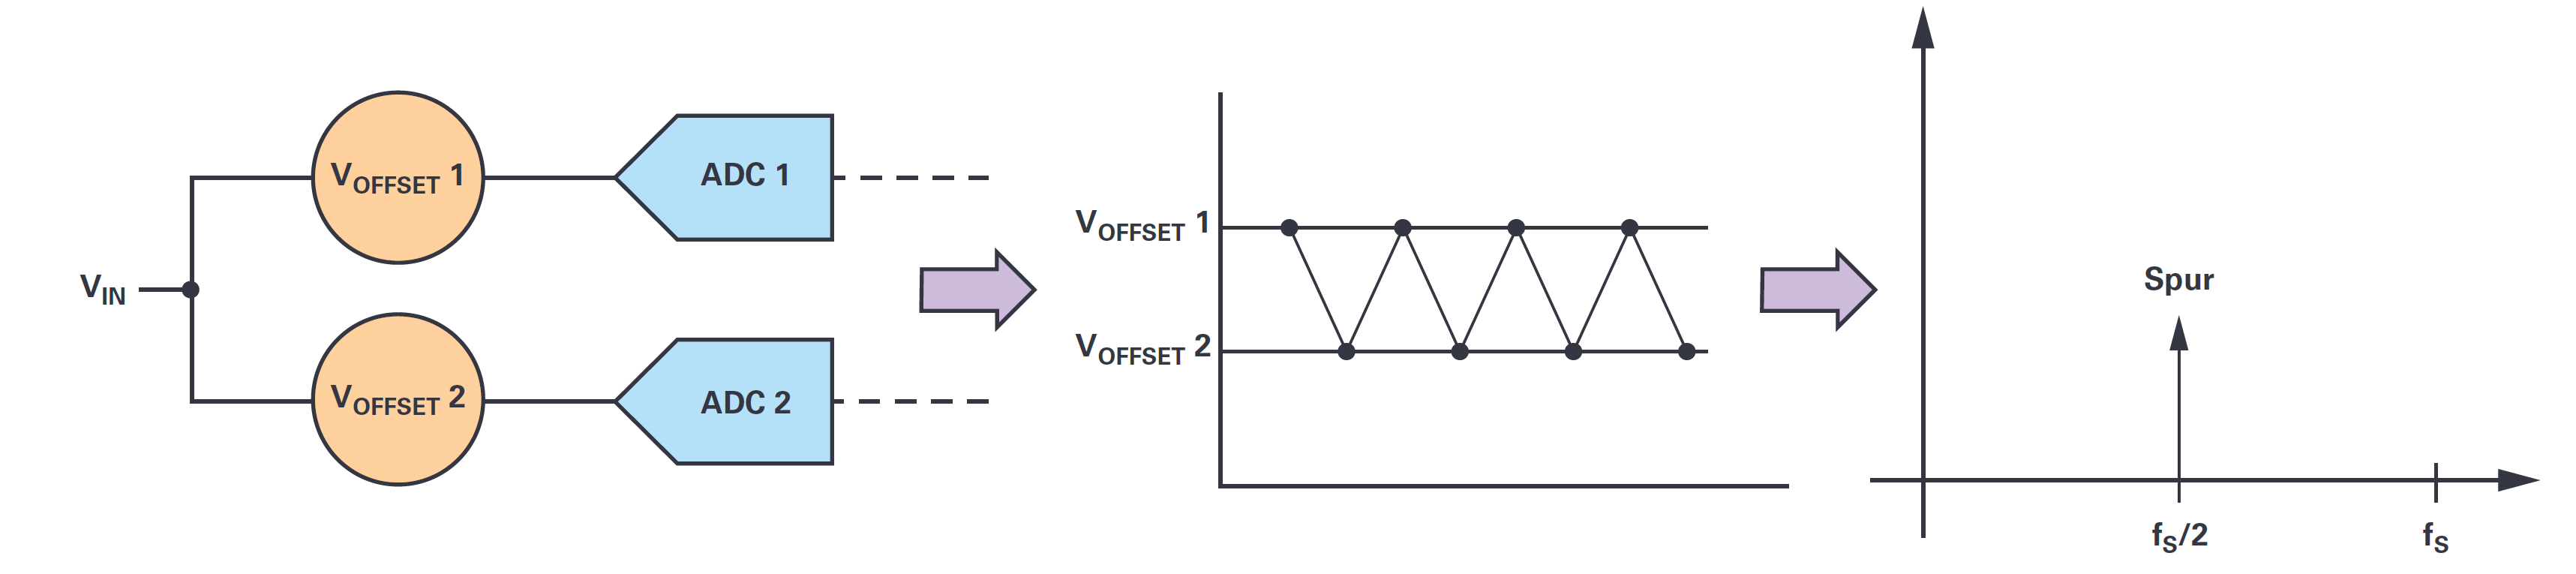
\includegraphics[width = \textwidth]{chap/03-newSys/img/interleaving//offset_mm}
	\caption{Offset-Mismatch in Interleaving \cite{Harris2019}}
	\label{fig:offset_mm}
\end{figure}

Besides of the offset also the gain of the converters can be mismatched. 
This \textit{gain mismatch} has a frequency component to it, which in case of an input signal of the frequency $f_{\text{in}}$ results in a spur at $\nicefrac{f_s}{2} \pm f_{\text{in}}$ (see \autoref{fig:gain_mm}). \cite{Harris2019}

\begin{figure}[tb]
	\centering
	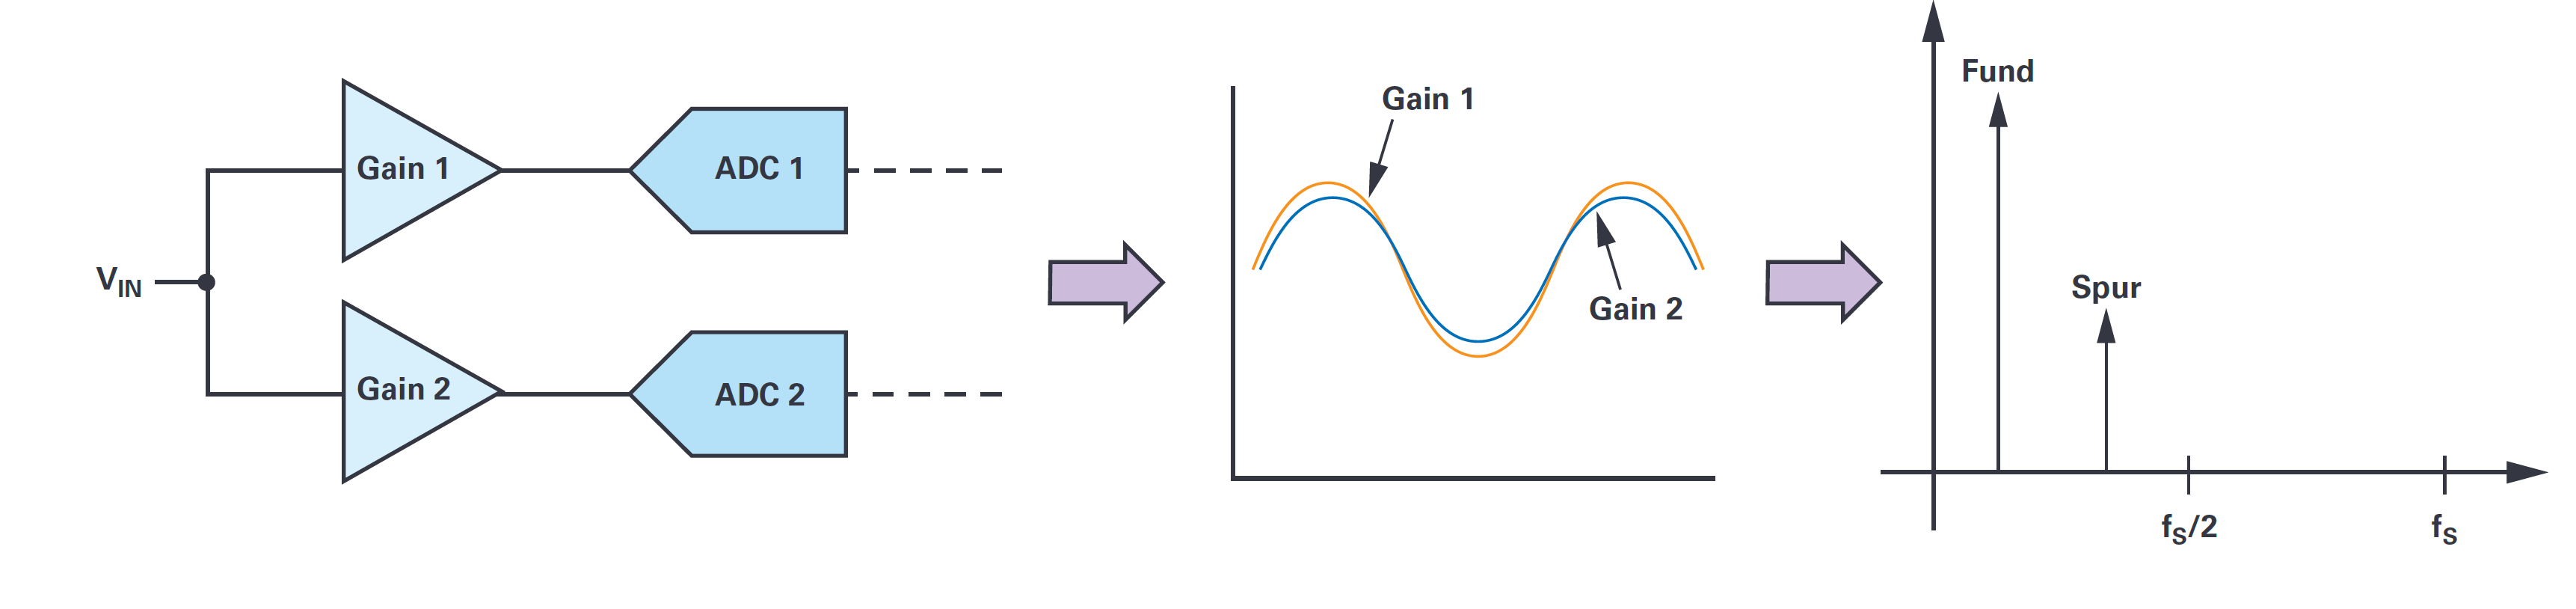
\includegraphics[width = \textwidth]{chap/03-newSys/img/interleaving/gain_mm}
	\caption{Gain-Mismatch in Interleaving \cite{Harris2019}}
	\label{fig:gain_mm}
\end{figure}

In the time domain, \textit{timing mismatch} due to group delay in the analog circuitry of the \gls{adc} and clock skew\footnote{Difference in arrival time of the clock signal at different components.} can occur. 
The group delay in analog circuitry can vary between the converters. 
The clock skew has on the one hand an aperture uncertainty component at each of the \glspl{adc}. 
On the other hand it has a component related to the accuracy of the clock phases, which are input to each converter. \cite{Harris2019} 
This mismatch also produces a spurious component at $\nicefrac{f_s}{2} \pm f_\text{in}$ (see \autoref{fig:timing_mm}).

\begin{figure}[tb]
	\centering
	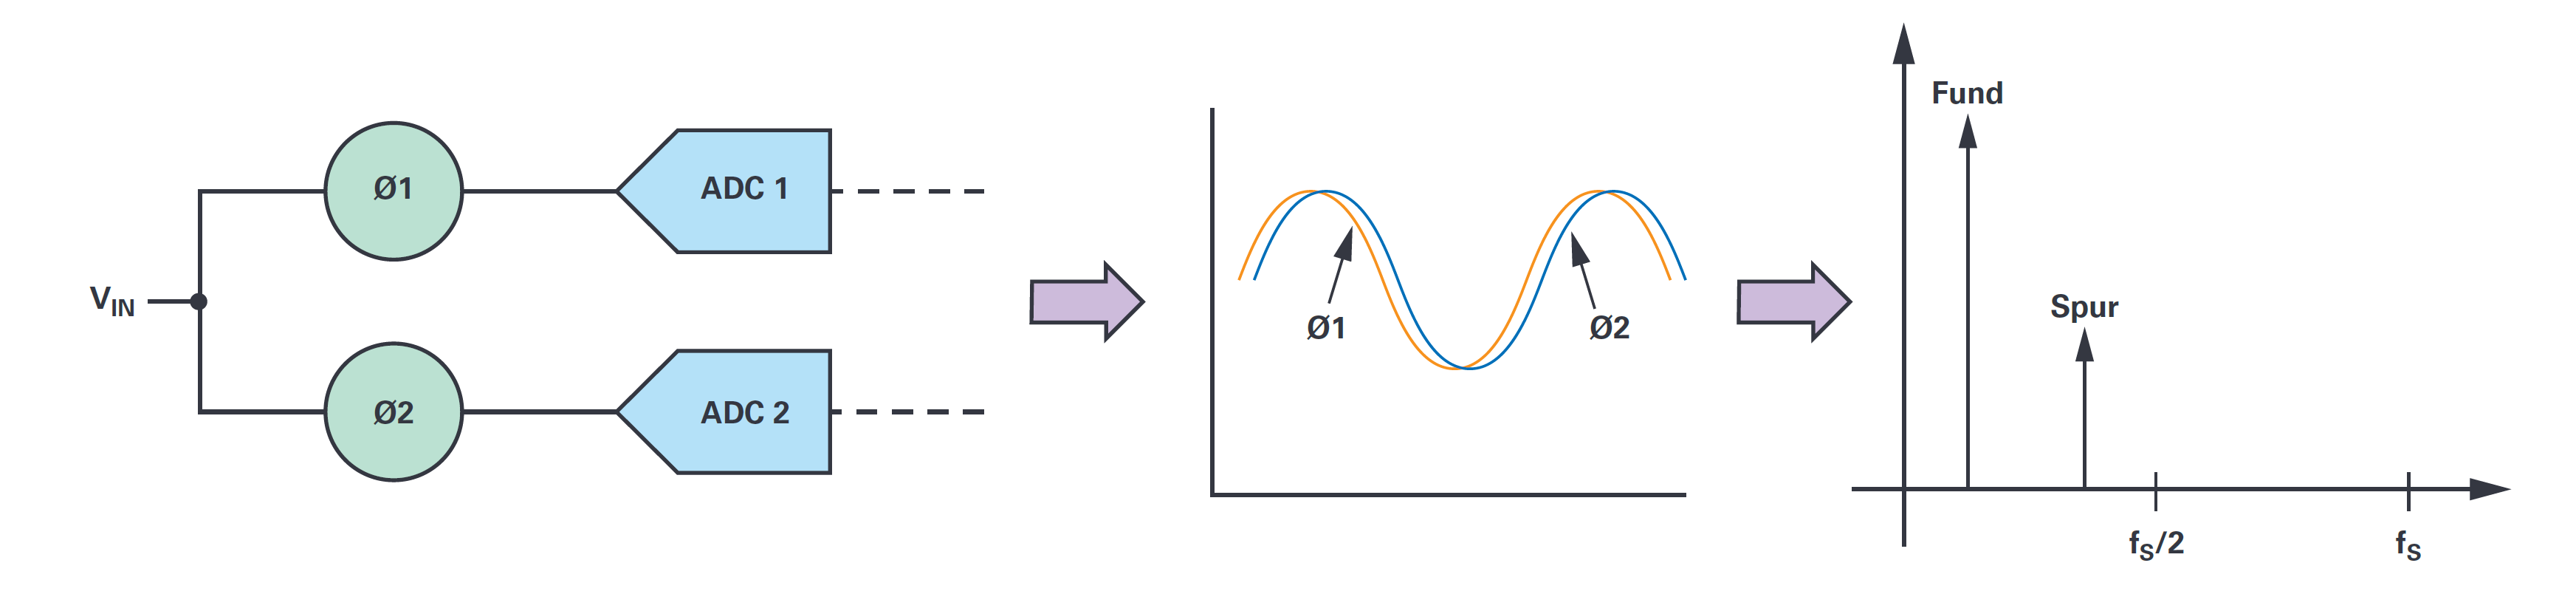
\includegraphics[width = \textwidth]{chap/03-newSys/img/interleaving/timing_mm}
	\caption{Timing-Mismatch in Interleaving \cite{Harris2019}}
	\label{fig:timing_mm}
\end{figure}

The last possible mismatch is the \textit{bandwidth mismatch}, which contains both gain and phase/frequency component (see \autoref{fig:bandwidth_mm}). 
Due to bandwidth mismatch, different gain values at different frequencies can be seen. 
An additional timing component causes different delays for signals at different frequencies through each \gls{adc}. 
Just like gain and timing mismatch, the bandwidth mismatch causes a spur at $\nicefrac{f_s}{2} \pm f_\text{in}$.

\begin{figure}[tb]
	\centering
	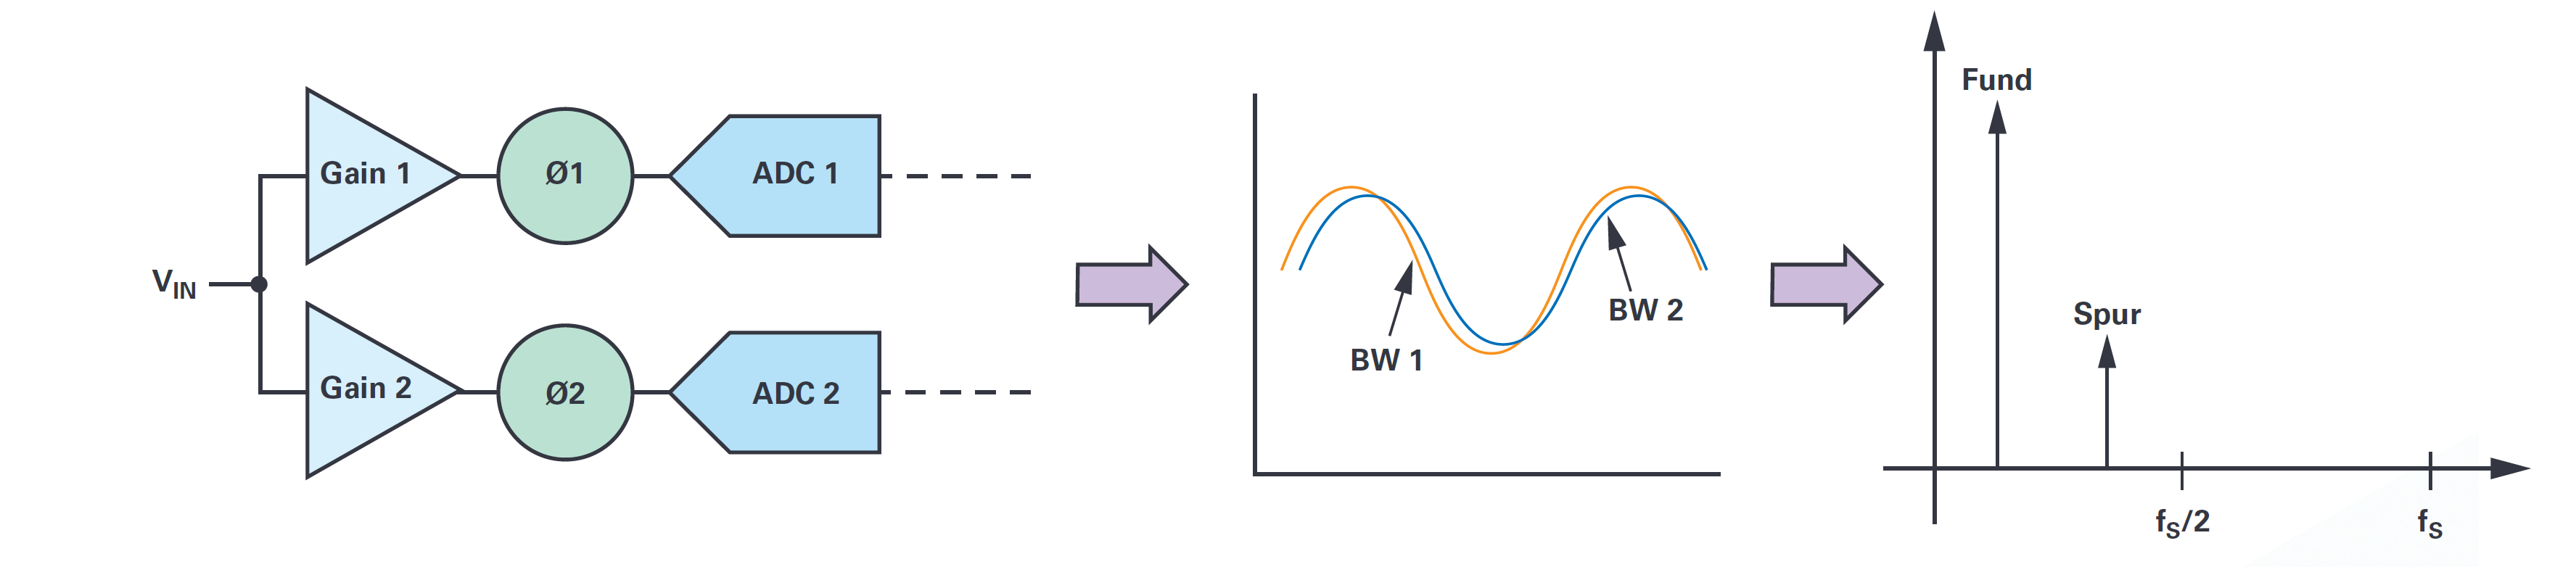
\includegraphics[width = \textwidth]{chap/03-newSys/img/interleaving/bandwidth_mm}
	\caption{Timing-Mismatch in Interleaving \cite{Harris2019}}
	\label{fig:bandwidth_mm}
\end{figure}
%todo zweimal timing mismatch

Due to the presented mismatches, a proper characterization of the \glspl{adc}. %todo hier fehlt was
The characterization is required in order to account for all systematical errors in the \glspl{adc} and to reduce the spurious components in the spectrum.
For this purpose, a circuit on the \gls{theresa} sampling board is foreseen, in order to provide the possibility to generate test signals from the readout card.

\subsubsection{Implementation}\label{ssec:interl_impl}
On the selected readout card for \gls{theresa}, 16 \glspl{adc} with a sampling rate up to \SI{2.5}{\GHz} are present.
In order to implement the time-interleaving method, an appropriate delay step size for the sample time has to be calculated.
To calculate the maximal step size possible can be calculated as follows: 
The \glspl{adc} on the read-out card sample at a maximal sample rate of \SI{2.5}{\giga\sample\per\second}, meaning during the time
\begin{equation}
	t_s = \frac{1}{\SI{2.5}{\giga \sample \per \second}} = \SI{400}{\pico \second}
\end{equation}
all 16 \glspl{adc} have to sample the signal one time.
This means, a delay step can not be greater than $\nicefrac{\SI{400}{\pico\second}}{16} = \SI{25}{\pico\second}$.
With this method, the maximal achievable sampling rate of the card is $16 \cdot \SI{2.5}{\giga\sample\per\second}  = \SI{40}{\giga\sample\per\second}$. 

On the selected readout card, sampling clock signals are not propagated individually to the respective \glspl{adc}.
The converters are grouped grouped together into tiles, each tile containing four converters.
One single reference clock signal is propagated to all tiles. 
To implement the optimal time-interleaving method with this card, four individual sampling clocks to all tiles shifted by \ang{90} would be necessary.
Analyzing the schematic of the readout board revealed however, that only two individual sampling clocks can be provided to the card.

Therefore, another approach needs to be considered.
\autoref{fig:THA} shows qualitatively the concept.
The main \SI{1}{\GHz} clock is propagated to the \glspl{tha}, which are in hold-mode when the clock signal is HIGH and in track-mode when the clock signal is LOW.
As shown in \autoref{fig:THA} the clock signal to each \gls{tha} is provided with a respective delay.
The maximal delay step size to cover the whole period of the clock is calculated by: 
\begin{equation}
	\frac{\SI{1}{\nano\second}}{16 \, \text{channels}} = \SI{62.5}{\pico\second}
\end{equation}

In some way, this implementation can therefore also be regarded as time-interleaving, as each \gls{tha} holds a different sample point in time, which can then be converted by the \glspl{adc}.
The two sampling clocks, indicated with ``ADC1'' and ``ADC2'', need the to be phase-shifted by \ang{180}. %todo ADC_1 statt ADC1?
In this way, an alternate clocking of the \glspl{adc} is made possible\footnote{As can be derived from the diagram, only the four respective \gls{adc} channels should be considered for signal conversion during one sampling point.}.

\begin{sidewaysfigure}[tbh]
	\centering
	\tikzexternaldisable
	\includegraphics[width = 0.8\textwidth]{chap/03-newSys/img/interleaving/interl_timing.tikz}
	\tikzexternalenable
	\caption[Track-And-Hold Timing diagram]{\gls{tha} Timing diagram. Shows the clocking of the \gls{tha} (HIGH = hold mode, LOW = track mode). Dashed line represents the sampling of the \gls{adc}.}
	\label{fig:THA}
\end{sidewaysfigure}

 
\subsection{Readout Card}\label{sec:selection}
The most important points to consider when choosing the readout card is its capability to handle high data-throughput, provide the possibility for user-defined firmware and control of the system.
This flexibility is provided by \gls{fpga}-based \glspl{soc}, which also integrate the required high-speed peripheral connections for data transfer.
An important point for \gls{theresa} is also to integrate the \glspl{adc} inside the \gls{soc}. 
The reason for this is illustrated in \autoref{fig:footprint}. 
In order to fulfill the requirements, the system would need a processing unit, an \gls{fpga} and a number of data converters (\gls{adc}/\gls{dac}).
Realizing this in discrete components results in a higher footprint, than integrating every component inside one \gls{ic}.

Integration of the necessary components inside an \gls{ic} also drastically reduces the complexity of the sampling board.
Implementing the data converters in a discrete way would result in a high number of interfaces/connections, especially for a high \gls{adc} resolution,  making expensive high pin count connectors necessary.
Integrating the converters inside the \gls{soc} therefore resolves these challenges.

The currently only commercially available system, meeting the mentioned requirements, is the Xilinx ZU49DR Zynq Ultrascale+ \gls{rfsoc}.
This \gls{soc} integrates 16 high-speed data converters (\glspl{adc} and \glspl{dac}), ARM processor cores and programmable logic (the \gls{fpga}).
An evaluation card, containing all necessary peripherals (optical interfaces, \gls{usb}, \dots) and integrating the \gls{rfsoc}, was chosen for the implementation of the \gls{theresa} system.
The card is described in detail in \autoref{chap:readout}.


\begin{figure}[tb]
	\centering
	\begin{subfigure}{0.5\textwidth}
		\centering
		\includegraphics{chap/03-newSys/img/footprint_1.tikz}  
		\caption{Discrete components}
		\label{fig:discreteComp}
	\end{subfigure}
	\\[4ex]
	\begin{subfigure}{0.5\textwidth}
		\centering
		\tikzexternaldisable
		\includegraphics{chap/03-newSys/img/footprint_2.tikz}  
		\caption{Integrated circuit}
		\tikzexternalenable
		\label{fig:integratedComp}
	\end{subfigure}
	\caption[Discrete components vs. IC]{Footprint of discrete components vs. footprint of \gls{ic} integrating the components}
	\label{fig:footprint}
\end{figure}